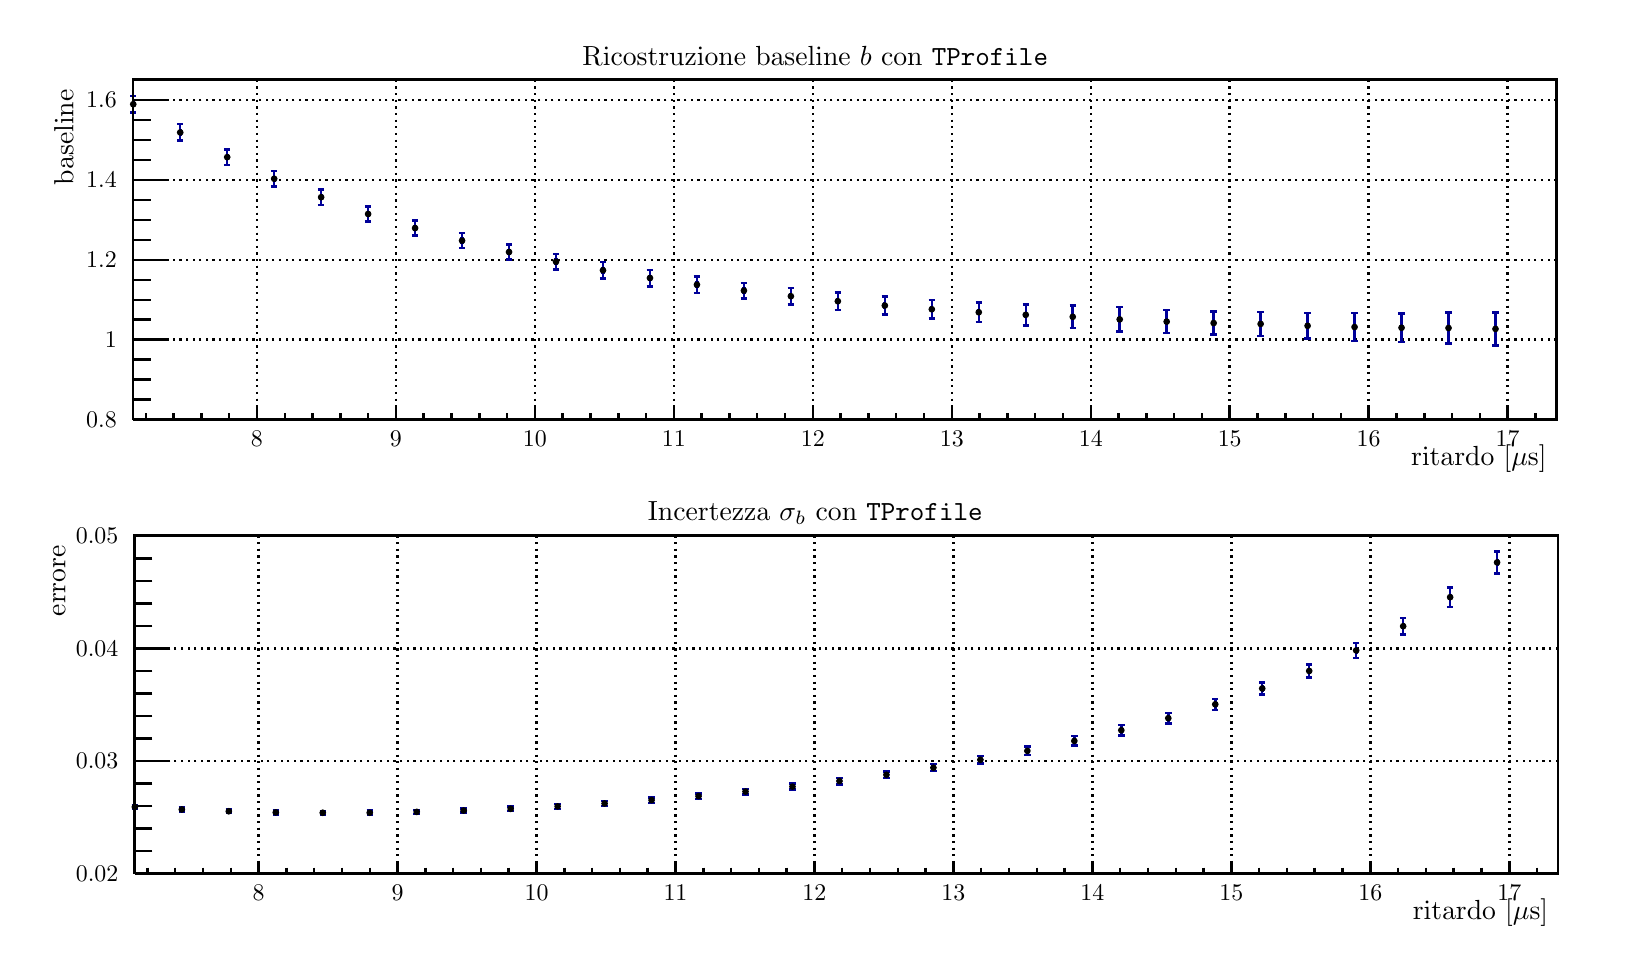
\begin{tikzpicture}
\pgfdeclareplotmark{cross} {
\pgfpathmoveto{\pgfpoint{-0.3\pgfplotmarksize}{\pgfplotmarksize}}
\pgfpathlineto{\pgfpoint{+0.3\pgfplotmarksize}{\pgfplotmarksize}}
\pgfpathlineto{\pgfpoint{+0.3\pgfplotmarksize}{0.3\pgfplotmarksize}}
\pgfpathlineto{\pgfpoint{+1\pgfplotmarksize}{0.3\pgfplotmarksize}}
\pgfpathlineto{\pgfpoint{+1\pgfplotmarksize}{-0.3\pgfplotmarksize}}
\pgfpathlineto{\pgfpoint{+0.3\pgfplotmarksize}{-0.3\pgfplotmarksize}}
\pgfpathlineto{\pgfpoint{+0.3\pgfplotmarksize}{-1.\pgfplotmarksize}}
\pgfpathlineto{\pgfpoint{-0.3\pgfplotmarksize}{-1.\pgfplotmarksize}}
\pgfpathlineto{\pgfpoint{-0.3\pgfplotmarksize}{-0.3\pgfplotmarksize}}
\pgfpathlineto{\pgfpoint{-1.\pgfplotmarksize}{-0.3\pgfplotmarksize}}
\pgfpathlineto{\pgfpoint{-1.\pgfplotmarksize}{0.3\pgfplotmarksize}}
\pgfpathlineto{\pgfpoint{-0.3\pgfplotmarksize}{0.3\pgfplotmarksize}}
\pgfpathclose
\pgfusepathqstroke
}
\pgfdeclareplotmark{cross*} {
\pgfpathmoveto{\pgfpoint{-0.3\pgfplotmarksize}{\pgfplotmarksize}}
\pgfpathlineto{\pgfpoint{+0.3\pgfplotmarksize}{\pgfplotmarksize}}
\pgfpathlineto{\pgfpoint{+0.3\pgfplotmarksize}{0.3\pgfplotmarksize}}
\pgfpathlineto{\pgfpoint{+1\pgfplotmarksize}{0.3\pgfplotmarksize}}
\pgfpathlineto{\pgfpoint{+1\pgfplotmarksize}{-0.3\pgfplotmarksize}}
\pgfpathlineto{\pgfpoint{+0.3\pgfplotmarksize}{-0.3\pgfplotmarksize}}
\pgfpathlineto{\pgfpoint{+0.3\pgfplotmarksize}{-1.\pgfplotmarksize}}
\pgfpathlineto{\pgfpoint{-0.3\pgfplotmarksize}{-1.\pgfplotmarksize}}
\pgfpathlineto{\pgfpoint{-0.3\pgfplotmarksize}{-0.3\pgfplotmarksize}}
\pgfpathlineto{\pgfpoint{-1.\pgfplotmarksize}{-0.3\pgfplotmarksize}}
\pgfpathlineto{\pgfpoint{-1.\pgfplotmarksize}{0.3\pgfplotmarksize}}
\pgfpathlineto{\pgfpoint{-0.3\pgfplotmarksize}{0.3\pgfplotmarksize}}
\pgfpathclose
\pgfusepathqfillstroke
}
\pgfdeclareplotmark{newstar} {
\pgfpathmoveto{\pgfqpoint{0pt}{\pgfplotmarksize}}
\pgfpathlineto{\pgfqpointpolar{44}{0.5\pgfplotmarksize}}
\pgfpathlineto{\pgfqpointpolar{18}{\pgfplotmarksize}}
\pgfpathlineto{\pgfqpointpolar{-20}{0.5\pgfplotmarksize}}
\pgfpathlineto{\pgfqpointpolar{-54}{\pgfplotmarksize}}
\pgfpathlineto{\pgfqpointpolar{-90}{0.5\pgfplotmarksize}}
\pgfpathlineto{\pgfqpointpolar{234}{\pgfplotmarksize}}
\pgfpathlineto{\pgfqpointpolar{198}{0.5\pgfplotmarksize}}
\pgfpathlineto{\pgfqpointpolar{162}{\pgfplotmarksize}}
\pgfpathlineto{\pgfqpointpolar{134}{0.5\pgfplotmarksize}}
\pgfpathclose
\pgfusepathqstroke
}
\pgfdeclareplotmark{newstar*} {
\pgfpathmoveto{\pgfqpoint{0pt}{\pgfplotmarksize}}
\pgfpathlineto{\pgfqpointpolar{44}{0.5\pgfplotmarksize}}
\pgfpathlineto{\pgfqpointpolar{18}{\pgfplotmarksize}}
\pgfpathlineto{\pgfqpointpolar{-20}{0.5\pgfplotmarksize}}
\pgfpathlineto{\pgfqpointpolar{-54}{\pgfplotmarksize}}
\pgfpathlineto{\pgfqpointpolar{-90}{0.5\pgfplotmarksize}}
\pgfpathlineto{\pgfqpointpolar{234}{\pgfplotmarksize}}
\pgfpathlineto{\pgfqpointpolar{198}{0.5\pgfplotmarksize}}
\pgfpathlineto{\pgfqpointpolar{162}{\pgfplotmarksize}}
\pgfpathlineto{\pgfqpointpolar{134}{0.5\pgfplotmarksize}}
\pgfpathclose
\pgfusepathqfillstroke
}
\definecolor{c}{rgb}{1,1,1};
\draw [color=c, fill=c] (0,0) rectangle (20,11.5542);
\draw [color=c, fill=c] (0.2,5.89264) rectangle (19.8,11.4387);
\draw [color=c, fill=c] (1.32924,6.58487) rectangle (19.407,10.8998);
\definecolor{c}{rgb}{0,0,0};
\draw [c,line width=0.9] (1.32924,6.58487) -- (1.32924,10.8998) -- (19.407,10.8998) -- (19.407,6.58487) -- (1.32924,6.58487);
\definecolor{c}{rgb}{1,1,1};
\draw [color=c, fill=c] (1.32924,6.58487) rectangle (19.407,10.8998);
\definecolor{c}{rgb}{0,0,0};
\draw [c,line width=0.9] (1.32924,6.58487) -- (1.32924,10.8998) -- (19.407,10.8998) -- (19.407,6.58487) -- (1.32924,6.58487);
\draw [c,line width=0.9] (1.32924,6.58487) -- (19.407,6.58487);
\draw [c,dash pattern=on 0.80pt off 1.60pt ,line width=0.9] (2.90505,10.8998) -- (2.90505,6.58487);
\draw [c,dash pattern=on 0.80pt off 1.60pt ,line width=0.9] (4.66989,10.8998) -- (4.66989,6.58487);
\draw [c,dash pattern=on 0.80pt off 1.60pt ,line width=0.9] (6.43474,10.8998) -- (6.43474,6.58487);
\draw [c,dash pattern=on 0.80pt off 1.60pt ,line width=0.9] (8.19958,10.8998) -- (8.19958,6.58487);
\draw [c,dash pattern=on 0.80pt off 1.60pt ,line width=0.9] (9.96442,10.8998) -- (9.96442,6.58487);
\draw [c,dash pattern=on 0.80pt off 1.60pt ,line width=0.9] (11.7293,10.8998) -- (11.7293,6.58487);
\draw [c,dash pattern=on 0.80pt off 1.60pt ,line width=0.9] (13.4941,10.8998) -- (13.4941,6.58487);
\draw [c,dash pattern=on 0.80pt off 1.60pt ,line width=0.9] (15.259,10.8998) -- (15.259,6.58487);
\draw [c,dash pattern=on 0.80pt off 1.60pt ,line width=0.9] (17.0238,10.8998) -- (17.0238,6.58487);
\draw [c,dash pattern=on 0.80pt off 1.60pt ,line width=0.9] (18.7886,10.8998) -- (18.7886,6.58487);
\draw [c,dash pattern=on 0.80pt off 1.60pt ,line width=0.9] (2.90505,10.8998) -- (2.90505,6.58487);
\draw [c,dash pattern=on 0.80pt off 1.60pt ,line width=0.9] (18.7886,10.8998) -- (18.7886,6.58487);
\draw [c,line width=0.9] (1.32924,6.58487) -- (1.32924,10.8998);
\draw [c,dash pattern=on 0.80pt off 1.60pt ,line width=0.9] (19.407,6.58487) -- (1.32924,6.58487);
\draw [c,dash pattern=on 0.80pt off 1.60pt ,line width=0.9] (19.407,7.59875) -- (1.32924,7.59875);
\draw [c,dash pattern=on 0.80pt off 1.60pt ,line width=0.9] (19.407,8.61263) -- (1.32924,8.61263);
\draw [c,dash pattern=on 0.80pt off 1.60pt ,line width=0.9] (19.407,9.62651) -- (1.32924,9.62651);
\draw [c,dash pattern=on 0.80pt off 1.60pt ,line width=0.9] (19.407,10.6404) -- (1.32924,10.6404);
\draw [c,dash pattern=on 0.80pt off 1.60pt ,line width=0.9] (19.407,10.6404) -- (1.32924,10.6404);
\definecolor{c}{rgb}{0,0,0.6};
\draw [c,line width=0.9] (1.33376,10.4835) -- (1.33376,10.5889);
\draw [c,line width=0.9] (1.33376,10.5889) -- (1.33376,10.6943);
\draw [c,line width=0.9] (1.32924,10.5889) -- (1.33376,10.5889);
\draw [c,line width=0.9] (1.33376,10.5889) -- (1.33828,10.5889);
\draw [c,line width=0.9] (1.29286,10.4835) -- (1.37466,10.4835);
\draw [c,line width=0.9] (1.29286,10.6943) -- (1.37466,10.6943);
\draw [c,line width=0.9] (1.32924,10.548) -- (1.32924,10.6298);
\draw [c,line width=0.9] (1.33828,10.548) -- (1.33828,10.6298);
\definecolor{c}{rgb}{0,0,0};
\foreach \P in {(1.33376,10.5889)}{\draw[mark options={color=c,fill=c},mark size=2.402402pt,mark=*,mark size=1pt] plot coordinates {\P};}
\definecolor{c}{rgb}{0,0,0.6};
\draw [c,line width=0.9] (1.93033,10.1261) -- (1.93033,10.2306);
\draw [c,line width=0.9] (1.93033,10.2306) -- (1.93033,10.3352);
\draw [c,line width=0.9] (1.92581,10.2306) -- (1.93033,10.2306);
\draw [c,line width=0.9] (1.93033,10.2306) -- (1.93485,10.2306);
\draw [c,line width=0.9] (1.88943,10.1261) -- (1.97123,10.1261);
\draw [c,line width=0.9] (1.88943,10.3352) -- (1.97123,10.3352);
\draw [c,line width=0.9] (1.92581,10.1897) -- (1.92581,10.2715);
\draw [c,line width=0.9] (1.93485,10.1897) -- (1.93485,10.2715);
\definecolor{c}{rgb}{0,0,0};
\foreach \P in {(1.93033,10.2306)}{\draw[mark options={color=c,fill=c},mark size=2.402402pt,mark=*,mark size=1pt] plot coordinates {\P};}
\definecolor{c}{rgb}{0,0,0.6};
\draw [c,line width=0.9] (2.52689,9.81788) -- (2.52689,9.91694);
\draw [c,line width=0.9] (2.52689,9.91694) -- (2.52689,10.016);
\draw [c,line width=0.9] (2.52237,9.91694) -- (2.52689,9.91694);
\draw [c,line width=0.9] (2.52689,9.91694) -- (2.53141,9.91694);
\draw [c,line width=0.9] (2.48599,9.81788) -- (2.56779,9.81788);
\draw [c,line width=0.9] (2.48599,10.016) -- (2.56779,10.016);
\draw [c,line width=0.9] (2.52237,9.87604) -- (2.52237,9.95784);
\draw [c,line width=0.9] (2.53141,9.87604) -- (2.53141,9.95784);
\definecolor{c}{rgb}{0,0,0};
\foreach \P in {(2.52689,9.91694)}{\draw[mark options={color=c,fill=c},mark size=2.402402pt,mark=*,mark size=1pt] plot coordinates {\P};}
\definecolor{c}{rgb}{0,0,0.6};
\draw [c,line width=0.9] (3.12346,9.54217) -- (3.12346,9.64229);
\draw [c,line width=0.9] (3.12346,9.64229) -- (3.12346,9.74242);
\draw [c,line width=0.9] (3.11894,9.64229) -- (3.12346,9.64229);
\draw [c,line width=0.9] (3.12346,9.64229) -- (3.12798,9.64229);
\draw [c,line width=0.9] (3.08256,9.54217) -- (3.16436,9.54217);
\draw [c,line width=0.9] (3.08256,9.74242) -- (3.16436,9.74242);
\draw [c,line width=0.9] (3.11894,9.60139) -- (3.11894,9.68319);
\draw [c,line width=0.9] (3.12798,9.60139) -- (3.12798,9.68319);
\definecolor{c}{rgb}{0,0,0};
\foreach \P in {(3.12346,9.64229)}{\draw[mark options={color=c,fill=c},mark size=2.402402pt,mark=*,mark size=1pt] plot coordinates {\P};}
\definecolor{c}{rgb}{0,0,0.6};
\draw [c,line width=0.9] (3.72002,9.31188) -- (3.72002,9.4082);
\draw [c,line width=0.9] (3.72002,9.4082) -- (3.72002,9.50451);
\draw [c,line width=0.9] (3.7155,9.4082) -- (3.72002,9.4082);
\draw [c,line width=0.9] (3.72002,9.4082) -- (3.72454,9.4082);
\draw [c,line width=0.9] (3.67912,9.31188) -- (3.76092,9.31188);
\draw [c,line width=0.9] (3.67912,9.50451) -- (3.76092,9.50451);
\draw [c,line width=0.9] (3.7155,9.3673) -- (3.7155,9.4491);
\draw [c,line width=0.9] (3.72454,9.3673) -- (3.72454,9.4491);
\definecolor{c}{rgb}{0,0,0};
\foreach \P in {(3.72002,9.4082)}{\draw[mark options={color=c,fill=c},mark size=2.402402pt,mark=*,mark size=1pt] plot coordinates {\P};}
\definecolor{c}{rgb}{0,0,0.6};
\draw [c,line width=0.9] (4.31659,9.09694) -- (4.31659,9.19491);
\draw [c,line width=0.9] (4.31659,9.19491) -- (4.31659,9.29287);
\draw [c,line width=0.9] (4.31207,9.19491) -- (4.31659,9.19491);
\draw [c,line width=0.9] (4.31659,9.19491) -- (4.3211,9.19491);
\draw [c,line width=0.9] (4.27569,9.09694) -- (4.35748,9.09694);
\draw [c,line width=0.9] (4.27569,9.29287) -- (4.35748,9.29287);
\draw [c,line width=0.9] (4.31207,9.15401) -- (4.31207,9.23581);
\draw [c,line width=0.9] (4.3211,9.15401) -- (4.3211,9.23581);
\definecolor{c}{rgb}{0,0,0};
\foreach \P in {(4.31659,9.19491)}{\draw[mark options={color=c,fill=c},mark size=2.402402pt,mark=*,mark size=1pt] plot coordinates {\P};}
\definecolor{c}{rgb}{0,0,0.6};
\draw [c,line width=0.9] (4.91315,8.91922) -- (4.91315,9.01586);
\draw [c,line width=0.9] (4.91315,9.01586) -- (4.91315,9.1125);
\draw [c,line width=0.9] (4.90863,9.01586) -- (4.91315,9.01586);
\draw [c,line width=0.9] (4.91315,9.01586) -- (4.91767,9.01586);
\draw [c,line width=0.9] (4.87225,8.91922) -- (4.95405,8.91922);
\draw [c,line width=0.9] (4.87225,9.1125) -- (4.95405,9.1125);
\draw [c,line width=0.9] (4.90863,8.97496) -- (4.90863,9.05676);
\draw [c,line width=0.9] (4.91767,8.97496) -- (4.91767,9.05676);
\definecolor{c}{rgb}{0,0,0};
\foreach \P in {(4.91315,9.01586)}{\draw[mark options={color=c,fill=c},mark size=2.402402pt,mark=*,mark size=1pt] plot coordinates {\P};}
\definecolor{c}{rgb}{0,0,0.6};
\draw [c,line width=0.9] (5.50971,8.76193) -- (5.50971,8.85636);
\draw [c,line width=0.9] (5.50971,8.85636) -- (5.50971,8.95079);
\draw [c,line width=0.9] (5.50519,8.85636) -- (5.50971,8.85636);
\draw [c,line width=0.9] (5.50971,8.85636) -- (5.51423,8.85636);
\draw [c,line width=0.9] (5.46881,8.76193) -- (5.55061,8.76193);
\draw [c,line width=0.9] (5.46881,8.95079) -- (5.55061,8.95079);
\draw [c,line width=0.9] (5.50519,8.81546) -- (5.50519,8.89726);
\draw [c,line width=0.9] (5.51423,8.81546) -- (5.51423,8.89726);
\definecolor{c}{rgb}{0,0,0};
\foreach \P in {(5.50971,8.85636)}{\draw[mark options={color=c,fill=c},mark size=2.402402pt,mark=*,mark size=1pt] plot coordinates {\P};}
\definecolor{c}{rgb}{0,0,0.6};
\draw [c,line width=0.9] (6.10628,8.61636) -- (6.10628,8.71203);
\draw [c,line width=0.9] (6.10628,8.71203) -- (6.10628,8.8077);
\draw [c,line width=0.9] (6.10176,8.71203) -- (6.10628,8.71203);
\draw [c,line width=0.9] (6.10628,8.71203) -- (6.1108,8.71203);
\draw [c,line width=0.9] (6.06538,8.61636) -- (6.14718,8.61636);
\draw [c,line width=0.9] (6.06538,8.8077) -- (6.14718,8.8077);
\draw [c,line width=0.9] (6.10176,8.67113) -- (6.10176,8.75293);
\draw [c,line width=0.9] (6.1108,8.67113) -- (6.1108,8.75293);
\definecolor{c}{rgb}{0,0,0};
\foreach \P in {(6.10628,8.71203)}{\draw[mark options={color=c,fill=c},mark size=2.402402pt,mark=*,mark size=1pt] plot coordinates {\P};}
\definecolor{c}{rgb}{0,0,0.6};
\draw [c,line width=0.9] (6.70284,8.48909) -- (6.70284,8.58885);
\draw [c,line width=0.9] (6.70284,8.58885) -- (6.70284,8.68862);
\draw [c,line width=0.9] (6.69832,8.58885) -- (6.70284,8.58885);
\draw [c,line width=0.9] (6.70284,8.58885) -- (6.70736,8.58885);
\draw [c,line width=0.9] (6.66194,8.48909) -- (6.74374,8.48909);
\draw [c,line width=0.9] (6.66194,8.68862) -- (6.74374,8.68862);
\draw [c,line width=0.9] (6.69832,8.54795) -- (6.69832,8.62975);
\draw [c,line width=0.9] (6.70736,8.54795) -- (6.70736,8.62975);
\definecolor{c}{rgb}{0,0,0};
\foreach \P in {(6.70284,8.58885)}{\draw[mark options={color=c,fill=c},mark size=2.402402pt,mark=*,mark size=1pt] plot coordinates {\P};}
\definecolor{c}{rgb}{0,0,0.6};
\draw [c,line width=0.9] (7.29941,8.3757) -- (7.29941,8.47992);
\draw [c,line width=0.9] (7.29941,8.47992) -- (7.29941,8.58413);
\draw [c,line width=0.9] (7.29489,8.47992) -- (7.29941,8.47992);
\draw [c,line width=0.9] (7.29941,8.47992) -- (7.30393,8.47992);
\draw [c,line width=0.9] (7.25851,8.3757) -- (7.34031,8.3757);
\draw [c,line width=0.9] (7.25851,8.58413) -- (7.34031,8.58413);
\draw [c,line width=0.9] (7.29489,8.43902) -- (7.29489,8.52082);
\draw [c,line width=0.9] (7.30393,8.43902) -- (7.30393,8.52082);
\definecolor{c}{rgb}{0,0,0};
\foreach \P in {(7.29941,8.47992)}{\draw[mark options={color=c,fill=c},mark size=2.402402pt,mark=*,mark size=1pt] plot coordinates {\P};}
\definecolor{c}{rgb}{0,0,0.6};
\draw [c,line width=0.9] (7.89597,8.27713) -- (7.89597,8.38191);
\draw [c,line width=0.9] (7.89597,8.38191) -- (7.89597,8.48669);
\draw [c,line width=0.9] (7.89145,8.38191) -- (7.89597,8.38191);
\draw [c,line width=0.9] (7.89597,8.38191) -- (7.90049,8.38191);
\draw [c,line width=0.9] (7.85507,8.27713) -- (7.93687,8.27713);
\draw [c,line width=0.9] (7.85507,8.48669) -- (7.93687,8.48669);
\draw [c,line width=0.9] (7.89145,8.34101) -- (7.89145,8.42281);
\draw [c,line width=0.9] (7.90049,8.34101) -- (7.90049,8.42281);
\definecolor{c}{rgb}{0,0,0};
\foreach \P in {(7.89597,8.38191)}{\draw[mark options={color=c,fill=c},mark size=2.402402pt,mark=*,mark size=1pt] plot coordinates {\P};}
\definecolor{c}{rgb}{0,0,0.6};
\draw [c,line width=0.9] (8.49254,8.19443) -- (8.49254,8.29674);
\draw [c,line width=0.9] (8.49254,8.29674) -- (8.49254,8.39905);
\draw [c,line width=0.9] (8.48802,8.29674) -- (8.49254,8.29674);
\draw [c,line width=0.9] (8.49254,8.29674) -- (8.49706,8.29674);
\draw [c,line width=0.9] (8.45164,8.19443) -- (8.53344,8.19443);
\draw [c,line width=0.9] (8.45164,8.39905) -- (8.53344,8.39905);
\draw [c,line width=0.9] (8.48802,8.25584) -- (8.48802,8.33764);
\draw [c,line width=0.9] (8.49706,8.25584) -- (8.49706,8.33764);
\definecolor{c}{rgb}{0,0,0};
\foreach \P in {(8.49254,8.29674)}{\draw[mark options={color=c,fill=c},mark size=2.402402pt,mark=*,mark size=1pt] plot coordinates {\P};}
\definecolor{c}{rgb}{0,0,0.6};
\draw [c,line width=0.9] (9.0891,8.12213) -- (9.0891,8.22176);
\draw [c,line width=0.9] (9.0891,8.22176) -- (9.0891,8.3214);
\draw [c,line width=0.9] (9.08458,8.22176) -- (9.0891,8.22176);
\draw [c,line width=0.9] (9.0891,8.22176) -- (9.09362,8.22176);
\draw [c,line width=0.9] (9.0482,8.12213) -- (9.13,8.12213);
\draw [c,line width=0.9] (9.0482,8.3214) -- (9.13,8.3214);
\draw [c,line width=0.9] (9.08458,8.18086) -- (9.08458,8.26266);
\draw [c,line width=0.9] (9.09362,8.18086) -- (9.09362,8.26266);
\definecolor{c}{rgb}{0,0,0};
\foreach \P in {(9.0891,8.22176)}{\draw[mark options={color=c,fill=c},mark size=2.402402pt,mark=*,mark size=1pt] plot coordinates {\P};}
\definecolor{c}{rgb}{0,0,0.6};
\draw [c,line width=0.9] (9.68566,8.04668) -- (9.68566,8.15047);
\draw [c,line width=0.9] (9.68566,8.15047) -- (9.68566,8.25426);
\draw [c,line width=0.9] (9.68115,8.15047) -- (9.68566,8.15047);
\draw [c,line width=0.9] (9.68566,8.15047) -- (9.69018,8.15047);
\draw [c,line width=0.9] (9.64476,8.04668) -- (9.72656,8.04668);
\draw [c,line width=0.9] (9.64476,8.25426) -- (9.72656,8.25426);
\draw [c,line width=0.9] (9.68115,8.10957) -- (9.68115,8.19137);
\draw [c,line width=0.9] (9.69018,8.10957) -- (9.69018,8.19137);
\definecolor{c}{rgb}{0,0,0};
\foreach \P in {(9.68566,8.15047)}{\draw[mark options={color=c,fill=c},mark size=2.402402pt,mark=*,mark size=1pt] plot coordinates {\P};}
\definecolor{c}{rgb}{0,0,0.6};
\draw [c,line width=0.9] (10.2822,7.97329) -- (10.2822,8.08689);
\draw [c,line width=0.9] (10.2822,8.08689) -- (10.2822,8.20049);
\draw [c,line width=0.9] (10.2777,8.08689) -- (10.2822,8.08689);
\draw [c,line width=0.9] (10.2822,8.08689) -- (10.2867,8.08689);
\draw [c,line width=0.9] (10.2413,7.97329) -- (10.3231,7.97329);
\draw [c,line width=0.9] (10.2413,8.20049) -- (10.3231,8.20049);
\draw [c,line width=0.9] (10.2777,8.04599) -- (10.2777,8.12779);
\draw [c,line width=0.9] (10.2867,8.04599) -- (10.2867,8.12779);
\definecolor{c}{rgb}{0,0,0};
\foreach \P in {(10.2822,8.08689)}{\draw[mark options={color=c,fill=c},mark size=2.402402pt,mark=*,mark size=1pt] plot coordinates {\P};}
\definecolor{c}{rgb}{0,0,0.6};
\draw [c,line width=0.9] (10.8788,7.91608) -- (10.8788,8.03204);
\draw [c,line width=0.9] (10.8788,8.03204) -- (10.8788,8.148);
\draw [c,line width=0.9] (10.8743,8.03204) -- (10.8788,8.03204);
\draw [c,line width=0.9] (10.8788,8.03204) -- (10.8833,8.03204);
\draw [c,line width=0.9] (10.8379,7.91608) -- (10.9197,7.91608);
\draw [c,line width=0.9] (10.8379,8.148) -- (10.9197,8.148);
\draw [c,line width=0.9] (10.8743,7.99114) -- (10.8743,8.07294);
\draw [c,line width=0.9] (10.8833,7.99114) -- (10.8833,8.07294);
\definecolor{c}{rgb}{0,0,0};
\foreach \P in {(10.8788,8.03204)}{\draw[mark options={color=c,fill=c},mark size=2.402402pt,mark=*,mark size=1pt] plot coordinates {\P};}
\definecolor{c}{rgb}{0,0,0.6};
\draw [c,line width=0.9] (11.4754,7.86893) -- (11.4754,7.98511);
\draw [c,line width=0.9] (11.4754,7.98511) -- (11.4754,8.10129);
\draw [c,line width=0.9] (11.4708,7.98511) -- (11.4754,7.98511);
\draw [c,line width=0.9] (11.4754,7.98511) -- (11.4799,7.98511);
\draw [c,line width=0.9] (11.4345,7.86893) -- (11.5163,7.86893);
\draw [c,line width=0.9] (11.4345,8.10129) -- (11.5163,8.10129);
\draw [c,line width=0.9] (11.4708,7.94421) -- (11.4708,8.02601);
\draw [c,line width=0.9] (11.4799,7.94421) -- (11.4799,8.02601);
\definecolor{c}{rgb}{0,0,0};
\foreach \P in {(11.4754,7.98511)}{\draw[mark options={color=c,fill=c},mark size=2.402402pt,mark=*,mark size=1pt] plot coordinates {\P};}
\definecolor{c}{rgb}{0,0,0.6};
\draw [c,line width=0.9] (12.0719,7.82338) -- (12.0719,7.94719);
\draw [c,line width=0.9] (12.0719,7.94719) -- (12.0719,8.07099);
\draw [c,line width=0.9] (12.0674,7.94719) -- (12.0719,7.94719);
\draw [c,line width=0.9] (12.0719,7.94719) -- (12.0764,7.94719);
\draw [c,line width=0.9] (12.031,7.82338) -- (12.1128,7.82338);
\draw [c,line width=0.9] (12.031,8.07099) -- (12.1128,8.07099);
\draw [c,line width=0.9] (12.0674,7.90629) -- (12.0674,7.98809);
\draw [c,line width=0.9] (12.0764,7.90629) -- (12.0764,7.98809);
\definecolor{c}{rgb}{0,0,0};
\foreach \P in {(12.0719,7.94719)}{\draw[mark options={color=c,fill=c},mark size=2.402402pt,mark=*,mark size=1pt] plot coordinates {\P};}
\definecolor{c}{rgb}{0,0,0.6};
\draw [c,line width=0.9] (12.6685,7.78063) -- (12.6685,7.91425);
\draw [c,line width=0.9] (12.6685,7.91425) -- (12.6685,8.04788);
\draw [c,line width=0.9] (12.664,7.91425) -- (12.6685,7.91425);
\draw [c,line width=0.9] (12.6685,7.91425) -- (12.673,7.91425);
\draw [c,line width=0.9] (12.6276,7.78063) -- (12.7094,7.78063);
\draw [c,line width=0.9] (12.6276,8.04788) -- (12.7094,8.04788);
\draw [c,line width=0.9] (12.664,7.87335) -- (12.664,7.95515);
\draw [c,line width=0.9] (12.673,7.87335) -- (12.673,7.95515);
\definecolor{c}{rgb}{0,0,0};
\foreach \P in {(12.6685,7.91425)}{\draw[mark options={color=c,fill=c},mark size=2.402402pt,mark=*,mark size=1pt] plot coordinates {\P};}
\definecolor{c}{rgb}{0,0,0.6};
\draw [c,line width=0.9] (13.2651,7.74632) -- (13.2651,7.8889);
\draw [c,line width=0.9] (13.2651,7.8889) -- (13.2651,8.03147);
\draw [c,line width=0.9] (13.2605,7.8889) -- (13.2651,7.8889);
\draw [c,line width=0.9] (13.2651,7.8889) -- (13.2696,7.8889);
\draw [c,line width=0.9] (13.2242,7.74632) -- (13.306,7.74632);
\draw [c,line width=0.9] (13.2242,8.03147) -- (13.306,8.03147);
\draw [c,line width=0.9] (13.2605,7.848) -- (13.2605,7.9298);
\draw [c,line width=0.9] (13.2696,7.848) -- (13.2696,7.9298);
\definecolor{c}{rgb}{0,0,0};
\foreach \P in {(13.2651,7.8889)}{\draw[mark options={color=c,fill=c},mark size=2.402402pt,mark=*,mark size=1pt] plot coordinates {\P};}
\definecolor{c}{rgb}{0,0,0.6};
\draw [c,line width=0.9] (13.8616,7.70106) -- (13.8616,7.85646);
\draw [c,line width=0.9] (13.8616,7.85646) -- (13.8616,8.01185);
\draw [c,line width=0.9] (13.8571,7.85646) -- (13.8616,7.85646);
\draw [c,line width=0.9] (13.8616,7.85646) -- (13.8661,7.85646);
\draw [c,line width=0.9] (13.8207,7.70106) -- (13.9025,7.70106);
\draw [c,line width=0.9] (13.8207,8.01185) -- (13.9025,8.01185);
\draw [c,line width=0.9] (13.8571,7.81556) -- (13.8571,7.89736);
\draw [c,line width=0.9] (13.8661,7.81556) -- (13.8661,7.89736);
\definecolor{c}{rgb}{0,0,0};
\foreach \P in {(13.8616,7.85646)}{\draw[mark options={color=c,fill=c},mark size=2.402402pt,mark=*,mark size=1pt] plot coordinates {\P};}
\definecolor{c}{rgb}{0,0,0.6};
\draw [c,line width=0.9] (14.4582,7.68137) -- (14.4582,7.82797);
\draw [c,line width=0.9] (14.4582,7.82797) -- (14.4582,7.97458);
\draw [c,line width=0.9] (14.4537,7.82797) -- (14.4582,7.82797);
\draw [c,line width=0.9] (14.4582,7.82797) -- (14.4627,7.82797);
\draw [c,line width=0.9] (14.4173,7.68137) -- (14.4991,7.68137);
\draw [c,line width=0.9] (14.4173,7.97458) -- (14.4991,7.97458);
\draw [c,line width=0.9] (14.4537,7.78707) -- (14.4537,7.86887);
\draw [c,line width=0.9] (14.4627,7.78707) -- (14.4627,7.86887);
\definecolor{c}{rgb}{0,0,0};
\foreach \P in {(14.4582,7.82797)}{\draw[mark options={color=c,fill=c},mark size=2.402402pt,mark=*,mark size=1pt] plot coordinates {\P};}
\definecolor{c}{rgb}{0,0,0.6};
\draw [c,line width=0.9] (15.0547,7.66396) -- (15.0547,7.80995);
\draw [c,line width=0.9] (15.0547,7.80995) -- (15.0547,7.95593);
\draw [c,line width=0.9] (15.0502,7.80995) -- (15.0547,7.80995);
\draw [c,line width=0.9] (15.0547,7.80995) -- (15.0593,7.80995);
\draw [c,line width=0.9] (15.0138,7.66396) -- (15.0956,7.66396);
\draw [c,line width=0.9] (15.0138,7.95593) -- (15.0956,7.95593);
\draw [c,line width=0.9] (15.0502,7.76904) -- (15.0502,7.85084);
\draw [c,line width=0.9] (15.0593,7.76904) -- (15.0593,7.85084);
\definecolor{c}{rgb}{0,0,0};
\foreach \P in {(15.0547,7.80995)}{\draw[mark options={color=c,fill=c},mark size=2.402402pt,mark=*,mark size=1pt] plot coordinates {\P};}
\definecolor{c}{rgb}{0,0,0.6};
\draw [c,line width=0.9] (15.6513,7.64422) -- (15.6513,7.7986);
\draw [c,line width=0.9] (15.6513,7.7986) -- (15.6513,7.95298);
\draw [c,line width=0.9] (15.6468,7.7986) -- (15.6513,7.7986);
\draw [c,line width=0.9] (15.6513,7.7986) -- (15.6558,7.7986);
\draw [c,line width=0.9] (15.6104,7.64422) -- (15.6922,7.64422);
\draw [c,line width=0.9] (15.6104,7.95298) -- (15.6922,7.95298);
\draw [c,line width=0.9] (15.6468,7.7577) -- (15.6468,7.8395);
\draw [c,line width=0.9] (15.6558,7.7577) -- (15.6558,7.8395);
\definecolor{c}{rgb}{0,0,0};
\foreach \P in {(15.6513,7.7986)}{\draw[mark options={color=c,fill=c},mark size=2.402402pt,mark=*,mark size=1pt] plot coordinates {\P};}
\definecolor{c}{rgb}{0,0,0.6};
\draw [c,line width=0.9] (16.2479,7.61304) -- (16.2479,7.77481);
\draw [c,line width=0.9] (16.2479,7.77481) -- (16.2479,7.93659);
\draw [c,line width=0.9] (16.2434,7.77481) -- (16.2479,7.77481);
\draw [c,line width=0.9] (16.2479,7.77481) -- (16.2524,7.77481);
\draw [c,line width=0.9] (16.207,7.61304) -- (16.2888,7.61304);
\draw [c,line width=0.9] (16.207,7.93659) -- (16.2888,7.93659);
\draw [c,line width=0.9] (16.2434,7.73391) -- (16.2434,7.81571);
\draw [c,line width=0.9] (16.2524,7.73391) -- (16.2524,7.81571);
\definecolor{c}{rgb}{0,0,0};
\foreach \P in {(16.2479,7.77481)}{\draw[mark options={color=c,fill=c},mark size=2.402402pt,mark=*,mark size=1pt] plot coordinates {\P};}
\definecolor{c}{rgb}{0,0,0.6};
\draw [c,line width=0.9] (16.8444,7.5825) -- (16.8444,7.75925);
\draw [c,line width=0.9] (16.8444,7.75925) -- (16.8444,7.936);
\draw [c,line width=0.9] (16.8399,7.75925) -- (16.8444,7.75925);
\draw [c,line width=0.9] (16.8444,7.75925) -- (16.849,7.75925);
\draw [c,line width=0.9] (16.8035,7.5825) -- (16.8853,7.5825);
\draw [c,line width=0.9] (16.8035,7.936) -- (16.8853,7.936);
\draw [c,line width=0.9] (16.8399,7.71835) -- (16.8399,7.80015);
\draw [c,line width=0.9] (16.849,7.71835) -- (16.849,7.80015);
\definecolor{c}{rgb}{0,0,0};
\foreach \P in {(16.8444,7.75925)}{\draw[mark options={color=c,fill=c},mark size=2.402402pt,mark=*,mark size=1pt] plot coordinates {\P};}
\definecolor{c}{rgb}{0,0,0.6};
\draw [c,line width=0.9] (17.441,7.56887) -- (17.441,7.75021);
\draw [c,line width=0.9] (17.441,7.75021) -- (17.441,7.93154);
\draw [c,line width=0.9] (17.4365,7.75021) -- (17.441,7.75021);
\draw [c,line width=0.9] (17.441,7.75021) -- (17.4455,7.75021);
\draw [c,line width=0.9] (17.4001,7.56887) -- (17.4819,7.56887);
\draw [c,line width=0.9] (17.4001,7.93154) -- (17.4819,7.93154);
\draw [c,line width=0.9] (17.4365,7.70931) -- (17.4365,7.79111);
\draw [c,line width=0.9] (17.4455,7.70931) -- (17.4455,7.79111);
\definecolor{c}{rgb}{0,0,0};
\foreach \P in {(17.441,7.75021)}{\draw[mark options={color=c,fill=c},mark size=2.402402pt,mark=*,mark size=1pt] plot coordinates {\P};}
\definecolor{c}{rgb}{0,0,0.6};
\draw [c,line width=0.9] (18.0376,7.54821) -- (18.0376,7.7469);
\draw [c,line width=0.9] (18.0376,7.7469) -- (18.0376,7.94559);
\draw [c,line width=0.9] (18.033,7.7469) -- (18.0376,7.7469);
\draw [c,line width=0.9] (18.0376,7.7469) -- (18.0421,7.7469);
\draw [c,line width=0.9] (17.9967,7.54821) -- (18.0785,7.54821);
\draw [c,line width=0.9] (17.9967,7.94559) -- (18.0785,7.94559);
\draw [c,line width=0.9] (18.033,7.706) -- (18.033,7.7878);
\draw [c,line width=0.9] (18.0421,7.706) -- (18.0421,7.7878);
\definecolor{c}{rgb}{0,0,0};
\foreach \P in {(18.0376,7.7469)}{\draw[mark options={color=c,fill=c},mark size=2.402402pt,mark=*,mark size=1pt] plot coordinates {\P};}
\definecolor{c}{rgb}{0,0,0.6};
\draw [c,line width=0.9] (18.6341,7.5241) -- (18.6341,7.73533);
\draw [c,line width=0.9] (18.6341,7.73533) -- (18.6341,7.94656);
\draw [c,line width=0.9] (18.6296,7.73533) -- (18.6341,7.73533);
\draw [c,line width=0.9] (18.6341,7.73533) -- (18.6387,7.73533);
\draw [c,line width=0.9] (18.5932,7.5241) -- (18.675,7.5241);
\draw [c,line width=0.9] (18.5932,7.94656) -- (18.675,7.94656);
\draw [c,line width=0.9] (18.6296,7.69443) -- (18.6296,7.77623);
\draw [c,line width=0.9] (18.6387,7.69443) -- (18.6387,7.77623);
\definecolor{c}{rgb}{0,0,0};
\foreach \P in {(18.6341,7.73533)}{\draw[mark options={color=c,fill=c},mark size=2.402402pt,mark=*,mark size=1pt] plot coordinates {\P};}
\draw [c,line width=0.9] (1.32924,6.58487) -- (19.407,6.58487);
\draw [anchor= east] (19.407,6.08794) node[scale=0.999947, color=c, rotate=0]{ritardo [$\mu$s]};
\draw [c,line width=0.9] (2.90505,6.73833) -- (2.90505,6.58487);
\draw [c,line width=0.9] (3.25802,6.6616) -- (3.25802,6.58487);
\draw [c,line width=0.9] (3.61099,6.6616) -- (3.61099,6.58487);
\draw [c,line width=0.9] (3.96396,6.6616) -- (3.96396,6.58487);
\draw [c,line width=0.9] (4.31693,6.6616) -- (4.31693,6.58487);
\draw [c,line width=0.9] (4.66989,6.73833) -- (4.66989,6.58487);
\draw [c,line width=0.9] (5.02286,6.6616) -- (5.02286,6.58487);
\draw [c,line width=0.9] (5.37583,6.6616) -- (5.37583,6.58487);
\draw [c,line width=0.9] (5.7288,6.6616) -- (5.7288,6.58487);
\draw [c,line width=0.9] (6.08177,6.6616) -- (6.08177,6.58487);
\draw [c,line width=0.9] (6.43474,6.73833) -- (6.43474,6.58487);
\draw [c,line width=0.9] (6.78771,6.6616) -- (6.78771,6.58487);
\draw [c,line width=0.9] (7.14067,6.6616) -- (7.14067,6.58487);
\draw [c,line width=0.9] (7.49364,6.6616) -- (7.49364,6.58487);
\draw [c,line width=0.9] (7.84661,6.6616) -- (7.84661,6.58487);
\draw [c,line width=0.9] (8.19958,6.73833) -- (8.19958,6.58487);
\draw [c,line width=0.9] (8.55255,6.6616) -- (8.55255,6.58487);
\draw [c,line width=0.9] (8.90552,6.6616) -- (8.90552,6.58487);
\draw [c,line width=0.9] (9.25849,6.6616) -- (9.25849,6.58487);
\draw [c,line width=0.9] (9.61145,6.6616) -- (9.61145,6.58487);
\draw [c,line width=0.9] (9.96442,6.73833) -- (9.96442,6.58487);
\draw [c,line width=0.9] (10.3174,6.6616) -- (10.3174,6.58487);
\draw [c,line width=0.9] (10.6704,6.6616) -- (10.6704,6.58487);
\draw [c,line width=0.9] (11.0233,6.6616) -- (11.0233,6.58487);
\draw [c,line width=0.9] (11.3763,6.6616) -- (11.3763,6.58487);
\draw [c,line width=0.9] (11.7293,6.73833) -- (11.7293,6.58487);
\draw [c,line width=0.9] (12.0822,6.6616) -- (12.0822,6.58487);
\draw [c,line width=0.9] (12.4352,6.6616) -- (12.4352,6.58487);
\draw [c,line width=0.9] (12.7882,6.6616) -- (12.7882,6.58487);
\draw [c,line width=0.9] (13.1411,6.6616) -- (13.1411,6.58487);
\draw [c,line width=0.9] (13.4941,6.73833) -- (13.4941,6.58487);
\draw [c,line width=0.9] (13.8471,6.6616) -- (13.8471,6.58487);
\draw [c,line width=0.9] (14.2,6.6616) -- (14.2,6.58487);
\draw [c,line width=0.9] (14.553,6.6616) -- (14.553,6.58487);
\draw [c,line width=0.9] (14.906,6.6616) -- (14.906,6.58487);
\draw [c,line width=0.9] (15.259,6.73833) -- (15.259,6.58487);
\draw [c,line width=0.9] (15.6119,6.6616) -- (15.6119,6.58487);
\draw [c,line width=0.9] (15.9649,6.6616) -- (15.9649,6.58487);
\draw [c,line width=0.9] (16.3179,6.6616) -- (16.3179,6.58487);
\draw [c,line width=0.9] (16.6708,6.6616) -- (16.6708,6.58487);
\draw [c,line width=0.9] (17.0238,6.73833) -- (17.0238,6.58487);
\draw [c,line width=0.9] (17.3768,6.6616) -- (17.3768,6.58487);
\draw [c,line width=0.9] (17.7297,6.6616) -- (17.7297,6.58487);
\draw [c,line width=0.9] (18.0827,6.6616) -- (18.0827,6.58487);
\draw [c,line width=0.9] (18.4357,6.6616) -- (18.4357,6.58487);
\draw [c,line width=0.9] (18.7886,6.73833) -- (18.7886,6.58487);
\draw [c,line width=0.9] (2.90505,6.73833) -- (2.90505,6.58487);
\draw [c,line width=0.9] (2.55208,6.6616) -- (2.55208,6.58487);
\draw [c,line width=0.9] (2.19911,6.6616) -- (2.19911,6.58487);
\draw [c,line width=0.9] (1.84615,6.6616) -- (1.84615,6.58487);
\draw [c,line width=0.9] (1.49318,6.6616) -- (1.49318,6.58487);
\draw [c,line width=0.9] (18.7886,6.73833) -- (18.7886,6.58487);
\draw [c,line width=0.9] (19.1416,6.6616) -- (19.1416,6.58487);
\draw [anchor=base] (2.90505,6.24656) node[scale=0.86359, color=c, rotate=0]{8};
\draw [anchor=base] (4.66989,6.24656) node[scale=0.86359, color=c, rotate=0]{9};
\draw [anchor=base] (6.43474,6.24656) node[scale=0.86359, color=c, rotate=0]{10};
\draw [anchor=base] (8.19958,6.24656) node[scale=0.86359, color=c, rotate=0]{11};
\draw [anchor=base] (9.96442,6.24656) node[scale=0.86359, color=c, rotate=0]{12};
\draw [anchor=base] (11.7293,6.24656) node[scale=0.86359, color=c, rotate=0]{13};
\draw [anchor=base] (13.4941,6.24656) node[scale=0.86359, color=c, rotate=0]{14};
\draw [anchor=base] (15.259,6.24656) node[scale=0.86359, color=c, rotate=0]{15};
\draw [anchor=base] (17.0238,6.24656) node[scale=0.86359, color=c, rotate=0]{16};
\draw [anchor=base] (18.7886,6.24656) node[scale=0.86359, color=c, rotate=0]{17};
\draw [c,line width=0.9] (1.32924,6.58487) -- (1.32924,10.8998);
\draw [anchor= east] (0.451163,10.8998) node[scale=0.999947, color=c, rotate=90]{baseline};
\draw [c,line width=0.9] (1.78672,6.58487) -- (1.32924,6.58487);
\draw [c,line width=0.9] (1.55798,6.83834) -- (1.32924,6.83834);
\draw [c,line width=0.9] (1.55798,7.09181) -- (1.32924,7.09181);
\draw [c,line width=0.9] (1.55798,7.34528) -- (1.32924,7.34528);
\draw [c,line width=0.9] (1.78672,7.59875) -- (1.32924,7.59875);
\draw [c,line width=0.9] (1.55798,7.85222) -- (1.32924,7.85222);
\draw [c,line width=0.9] (1.55798,8.10569) -- (1.32924,8.10569);
\draw [c,line width=0.9] (1.55798,8.35916) -- (1.32924,8.35916);
\draw [c,line width=0.9] (1.78672,8.61263) -- (1.32924,8.61263);
\draw [c,line width=0.9] (1.55798,8.8661) -- (1.32924,8.8661);
\draw [c,line width=0.9] (1.55798,9.11957) -- (1.32924,9.11957);
\draw [c,line width=0.9] (1.55798,9.37304) -- (1.32924,9.37304);
\draw [c,line width=0.9] (1.78672,9.62651) -- (1.32924,9.62651);
\draw [c,line width=0.9] (1.55798,9.87998) -- (1.32924,9.87998);
\draw [c,line width=0.9] (1.55798,10.1335) -- (1.32924,10.1335);
\draw [c,line width=0.9] (1.55798,10.3869) -- (1.32924,10.3869);
\draw [c,line width=0.9] (1.78672,10.6404) -- (1.32924,10.6404);
\draw [c,line width=0.9] (1.78672,10.6404) -- (1.32924,10.6404);
\draw [c,line width=0.9] (1.55798,10.8939) -- (1.32924,10.8939);
\draw [anchor= east] (1.23124,6.58487) node[scale=0.86359, color=c, rotate=0]{0.8};
\draw [anchor= east] (1.23124,7.59875) node[scale=0.86359, color=c, rotate=0]{1};
\draw [anchor= east] (1.23124,8.61263) node[scale=0.86359, color=c, rotate=0]{1.2};
\draw [anchor= east] (1.23124,9.62651) node[scale=0.86359, color=c, rotate=0]{1.4};
\draw [anchor= east] (1.23124,10.6404) node[scale=0.86359, color=c, rotate=0]{1.6};
\draw (9.9955,11.2053) node[scale=0.999947, color=c, rotate=0]{Ricostruzione baseline $b$ con \texttt{TProfile}};
\definecolor{c}{rgb}{1,1,1};
\draw [color=c, fill=c] (0.2,0.115542) rectangle (19.8,5.66155);
\draw [color=c, fill=c] (1.34969,0.817996) rectangle (19.4274,5.11247);
\definecolor{c}{rgb}{0,0,0};
\draw [c,line width=0.9] (1.34969,0.817996) -- (1.34969,5.11247) -- (19.4274,5.11247) -- (19.4274,0.817996) -- (1.34969,0.817996);
\definecolor{c}{rgb}{1,1,1};
\draw [color=c, fill=c] (1.34969,0.817996) rectangle (19.4274,5.11247);
\definecolor{c}{rgb}{0,0,0};
\draw [c,line width=0.9] (1.34969,0.817996) -- (1.34969,5.11247) -- (19.4274,5.11247) -- (19.4274,0.817996) -- (1.34969,0.817996);
\draw [c,line width=0.9] (1.34969,0.817996) -- (19.4274,0.817996);
\draw [c,dash pattern=on 0.80pt off 1.60pt ,line width=0.9] (2.9255,5.11247) -- (2.9255,0.817996);
\draw [c,dash pattern=on 0.80pt off 1.60pt ,line width=0.9] (4.69034,5.11247) -- (4.69034,0.817996);
\draw [c,dash pattern=on 0.80pt off 1.60pt ,line width=0.9] (6.45519,5.11247) -- (6.45519,0.817996);
\draw [c,dash pattern=on 0.80pt off 1.60pt ,line width=0.9] (8.22003,5.11247) -- (8.22003,0.817996);
\draw [c,dash pattern=on 0.80pt off 1.60pt ,line width=0.9] (9.98487,5.11247) -- (9.98487,0.817996);
\draw [c,dash pattern=on 0.80pt off 1.60pt ,line width=0.9] (11.7497,5.11247) -- (11.7497,0.817996);
\draw [c,dash pattern=on 0.80pt off 1.60pt ,line width=0.9] (13.5146,5.11247) -- (13.5146,0.817996);
\draw [c,dash pattern=on 0.80pt off 1.60pt ,line width=0.9] (15.2794,5.11247) -- (15.2794,0.817996);
\draw [c,dash pattern=on 0.80pt off 1.60pt ,line width=0.9] (17.0442,5.11247) -- (17.0442,0.817996);
\draw [c,dash pattern=on 0.80pt off 1.60pt ,line width=0.9] (18.8091,5.11247) -- (18.8091,0.817996);
\draw [c,dash pattern=on 0.80pt off 1.60pt ,line width=0.9] (2.9255,5.11247) -- (2.9255,0.817996);
\draw [c,dash pattern=on 0.80pt off 1.60pt ,line width=0.9] (18.8091,5.11247) -- (18.8091,0.817996);
\draw [c,line width=0.9] (1.34969,0.817996) -- (1.34969,5.11247);
\draw [c,dash pattern=on 0.80pt off 1.60pt ,line width=0.9] (19.4274,0.817996) -- (1.34969,0.817996);
\draw [c,dash pattern=on 0.80pt off 1.60pt ,line width=0.9] (19.4274,2.24693) -- (1.34969,2.24693);
\draw [c,dash pattern=on 0.80pt off 1.60pt ,line width=0.9] (19.4274,3.67587) -- (1.34969,3.67587);
\draw [c,dash pattern=on 0.80pt off 1.60pt ,line width=0.9] (19.4274,5.1048) -- (1.34969,5.1048);
\draw [c,dash pattern=on 0.80pt off 1.60pt ,line width=0.9] (19.4274,5.1048) -- (1.34969,5.1048);
\definecolor{c}{rgb}{0,0,0.6};
\draw [c,line width=0.9] (1.35421,1.64001) -- (1.35421,1.66414);
\draw [c,line width=0.9] (1.35421,1.66414) -- (1.35421,1.68827);
\draw [c,line width=0.9] (1.34969,1.66414) -- (1.35421,1.66414);
\draw [c,line width=0.9] (1.35421,1.66414) -- (1.35873,1.66414);
\draw [c,line width=0.9] (1.31331,1.64001) -- (1.39511,1.64001);
\draw [c,line width=0.9] (1.31331,1.68827) -- (1.39511,1.68827);
\draw [c,line width=0.9] (1.34969,1.62324) -- (1.34969,1.70504);
\draw [c,line width=0.9] (1.35873,1.62324) -- (1.35873,1.70504);
\definecolor{c}{rgb}{0,0,0};
\foreach \P in {(1.35421,1.66414)}{\draw[mark options={color=c,fill=c},mark size=2.402402pt,mark=*,mark size=1pt] plot coordinates {\P};}
\definecolor{c}{rgb}{0,0,0.6};
\draw [c,line width=0.9] (1.95078,1.60757) -- (1.95078,1.63246);
\draw [c,line width=0.9] (1.95078,1.63246) -- (1.95078,1.65734);
\draw [c,line width=0.9] (1.94626,1.63246) -- (1.95078,1.63246);
\draw [c,line width=0.9] (1.95078,1.63246) -- (1.9553,1.63246);
\draw [c,line width=0.9] (1.90988,1.60757) -- (1.99168,1.60757);
\draw [c,line width=0.9] (1.90988,1.65734) -- (1.99168,1.65734);
\draw [c,line width=0.9] (1.94626,1.59156) -- (1.94626,1.67336);
\draw [c,line width=0.9] (1.9553,1.59156) -- (1.9553,1.67336);
\definecolor{c}{rgb}{0,0,0};
\foreach \P in {(1.95078,1.63246)}{\draw[mark options={color=c,fill=c},mark size=2.402402pt,mark=*,mark size=1pt] plot coordinates {\P};}
\definecolor{c}{rgb}{0,0,0.6};
\draw [c,line width=0.9] (2.54734,1.58525) -- (2.54734,1.60963);
\draw [c,line width=0.9] (2.54734,1.60963) -- (2.54734,1.63402);
\draw [c,line width=0.9] (2.54282,1.60963) -- (2.54734,1.60963);
\draw [c,line width=0.9] (2.54734,1.60963) -- (2.55186,1.60963);
\draw [c,line width=0.9] (2.50644,1.58525) -- (2.58824,1.58525);
\draw [c,line width=0.9] (2.50644,1.63402) -- (2.58824,1.63402);
\draw [c,line width=0.9] (2.54282,1.56873) -- (2.54282,1.65053);
\draw [c,line width=0.9] (2.55186,1.56873) -- (2.55186,1.65053);
\definecolor{c}{rgb}{0,0,0};
\foreach \P in {(2.54734,1.60963)}{\draw[mark options={color=c,fill=c},mark size=2.402402pt,mark=*,mark size=1pt] plot coordinates {\P};}
\definecolor{c}{rgb}{0,0,0.6};
\draw [c,line width=0.9] (3.14391,1.56966) -- (3.14391,1.59524);
\draw [c,line width=0.9] (3.14391,1.59524) -- (3.14391,1.62083);
\draw [c,line width=0.9] (3.13939,1.59524) -- (3.14391,1.59524);
\draw [c,line width=0.9] (3.14391,1.59524) -- (3.14843,1.59524);
\draw [c,line width=0.9] (3.10301,1.56966) -- (3.18481,1.56966);
\draw [c,line width=0.9] (3.10301,1.62083) -- (3.18481,1.62083);
\draw [c,line width=0.9] (3.13939,1.55434) -- (3.13939,1.63614);
\draw [c,line width=0.9] (3.14843,1.55434) -- (3.14843,1.63614);
\definecolor{c}{rgb}{0,0,0};
\foreach \P in {(3.14391,1.59524)}{\draw[mark options={color=c,fill=c},mark size=2.402402pt,mark=*,mark size=1pt] plot coordinates {\P};}
\definecolor{c}{rgb}{0,0,0.6};
\draw [c,line width=0.9] (3.74047,1.56525) -- (3.74047,1.59061);
\draw [c,line width=0.9] (3.74047,1.59061) -- (3.74047,1.61598);
\draw [c,line width=0.9] (3.73595,1.59061) -- (3.74047,1.59061);
\draw [c,line width=0.9] (3.74047,1.59061) -- (3.74499,1.59061);
\draw [c,line width=0.9] (3.69957,1.56525) -- (3.78137,1.56525);
\draw [c,line width=0.9] (3.69957,1.61598) -- (3.78137,1.61598);
\draw [c,line width=0.9] (3.73595,1.54971) -- (3.73595,1.63151);
\draw [c,line width=0.9] (3.74499,1.54971) -- (3.74499,1.63151);
\definecolor{c}{rgb}{0,0,0};
\foreach \P in {(3.74047,1.59061)}{\draw[mark options={color=c,fill=c},mark size=2.402402pt,mark=*,mark size=1pt] plot coordinates {\P};}
\definecolor{c}{rgb}{0,0,0.6};
\draw [c,line width=0.9] (4.33703,1.56458) -- (4.33703,1.59134);
\draw [c,line width=0.9] (4.33703,1.59134) -- (4.33703,1.6181);
\draw [c,line width=0.9] (4.33252,1.59134) -- (4.33703,1.59134);
\draw [c,line width=0.9] (4.33703,1.59134) -- (4.34155,1.59134);
\draw [c,line width=0.9] (4.29613,1.56458) -- (4.37793,1.56458);
\draw [c,line width=0.9] (4.29613,1.6181) -- (4.37793,1.6181);
\draw [c,line width=0.9] (4.33252,1.55044) -- (4.33252,1.63224);
\draw [c,line width=0.9] (4.34155,1.55044) -- (4.34155,1.63224);
\definecolor{c}{rgb}{0,0,0};
\foreach \P in {(4.33703,1.59134)}{\draw[mark options={color=c,fill=c},mark size=2.402402pt,mark=*,mark size=1pt] plot coordinates {\P};}
\definecolor{c}{rgb}{0,0,0.6};
\draw [c,line width=0.9] (4.9336,1.57475) -- (4.9336,1.60175);
\draw [c,line width=0.9] (4.9336,1.60175) -- (4.9336,1.62874);
\draw [c,line width=0.9] (4.92908,1.60175) -- (4.9336,1.60175);
\draw [c,line width=0.9] (4.9336,1.60175) -- (4.93812,1.60175);
\draw [c,line width=0.9] (4.8927,1.57475) -- (4.9745,1.57475);
\draw [c,line width=0.9] (4.8927,1.62874) -- (4.9745,1.62874);
\draw [c,line width=0.9] (4.92908,1.56085) -- (4.92908,1.64265);
\draw [c,line width=0.9] (4.93812,1.56085) -- (4.93812,1.64265);
\definecolor{c}{rgb}{0,0,0};
\foreach \P in {(4.9336,1.60175)}{\draw[mark options={color=c,fill=c},mark size=2.402402pt,mark=*,mark size=1pt] plot coordinates {\P};}
\definecolor{c}{rgb}{0,0,0.6};
\draw [c,line width=0.9] (5.53016,1.59125) -- (5.53016,1.6185);
\draw [c,line width=0.9] (5.53016,1.6185) -- (5.53016,1.64574);
\draw [c,line width=0.9] (5.52564,1.6185) -- (5.53016,1.6185);
\draw [c,line width=0.9] (5.53016,1.6185) -- (5.53468,1.6185);
\draw [c,line width=0.9] (5.48926,1.59125) -- (5.57106,1.59125);
\draw [c,line width=0.9] (5.48926,1.64574) -- (5.57106,1.64574);
\draw [c,line width=0.9] (5.52564,1.5776) -- (5.52564,1.6594);
\draw [c,line width=0.9] (5.53468,1.5776) -- (5.53468,1.6594);
\definecolor{c}{rgb}{0,0,0};
\foreach \P in {(5.53016,1.6185)}{\draw[mark options={color=c,fill=c},mark size=2.402402pt,mark=*,mark size=1pt] plot coordinates {\P};}
\definecolor{c}{rgb}{0,0,0.6};
\draw [c,line width=0.9] (6.12673,1.61223) -- (6.12673,1.64088);
\draw [c,line width=0.9] (6.12673,1.64088) -- (6.12673,1.66952);
\draw [c,line width=0.9] (6.12221,1.64088) -- (6.12673,1.64088);
\draw [c,line width=0.9] (6.12673,1.64088) -- (6.13125,1.64088);
\draw [c,line width=0.9] (6.08583,1.61223) -- (6.16763,1.61223);
\draw [c,line width=0.9] (6.08583,1.66952) -- (6.16763,1.66952);
\draw [c,line width=0.9] (6.12221,1.59998) -- (6.12221,1.68178);
\draw [c,line width=0.9] (6.13125,1.59998) -- (6.13125,1.68178);
\definecolor{c}{rgb}{0,0,0};
\foreach \P in {(6.12673,1.64088)}{\draw[mark options={color=c,fill=c},mark size=2.402402pt,mark=*,mark size=1pt] plot coordinates {\P};}
\definecolor{c}{rgb}{0,0,0.6};
\draw [c,line width=0.9] (6.72329,1.6407) -- (6.72329,1.67126);
\draw [c,line width=0.9] (6.72329,1.67126) -- (6.72329,1.70181);
\draw [c,line width=0.9] (6.71877,1.67126) -- (6.72329,1.67126);
\draw [c,line width=0.9] (6.72329,1.67126) -- (6.72781,1.67126);
\draw [c,line width=0.9] (6.68239,1.6407) -- (6.76419,1.6407);
\draw [c,line width=0.9] (6.68239,1.70181) -- (6.76419,1.70181);
\draw [c,line width=0.9] (6.71877,1.63036) -- (6.71877,1.71216);
\draw [c,line width=0.9] (6.72781,1.63036) -- (6.72781,1.71216);
\definecolor{c}{rgb}{0,0,0};
\foreach \P in {(6.72329,1.67126)}{\draw[mark options={color=c,fill=c},mark size=2.402402pt,mark=*,mark size=1pt] plot coordinates {\P};}
\definecolor{c}{rgb}{0,0,0.6};
\draw [c,line width=0.9] (7.31986,1.67546) -- (7.31986,1.70819);
\draw [c,line width=0.9] (7.31986,1.70819) -- (7.31986,1.74092);
\draw [c,line width=0.9] (7.31534,1.70819) -- (7.31986,1.70819);
\draw [c,line width=0.9] (7.31986,1.70819) -- (7.32438,1.70819);
\draw [c,line width=0.9] (7.27896,1.67546) -- (7.36076,1.67546);
\draw [c,line width=0.9] (7.27896,1.74092) -- (7.36076,1.74092);
\draw [c,line width=0.9] (7.31534,1.66729) -- (7.31534,1.74909);
\draw [c,line width=0.9] (7.32438,1.66729) -- (7.32438,1.74909);
\definecolor{c}{rgb}{0,0,0};
\foreach \P in {(7.31986,1.70819)}{\draw[mark options={color=c,fill=c},mark size=2.402402pt,mark=*,mark size=1pt] plot coordinates {\P};}
\definecolor{c}{rgb}{0,0,0.6};
\draw [c,line width=0.9] (7.91642,1.71736) -- (7.91642,1.75125);
\draw [c,line width=0.9] (7.91642,1.75125) -- (7.91642,1.78514);
\draw [c,line width=0.9] (7.9119,1.75125) -- (7.91642,1.75125);
\draw [c,line width=0.9] (7.91642,1.75125) -- (7.92094,1.75125);
\draw [c,line width=0.9] (7.87552,1.71736) -- (7.95732,1.71736);
\draw [c,line width=0.9] (7.87552,1.78514) -- (7.95732,1.78514);
\draw [c,line width=0.9] (7.9119,1.71035) -- (7.9119,1.79215);
\draw [c,line width=0.9] (7.92094,1.71035) -- (7.92094,1.79215);
\definecolor{c}{rgb}{0,0,0};
\foreach \P in {(7.91642,1.75125)}{\draw[mark options={color=c,fill=c},mark size=2.402402pt,mark=*,mark size=1pt] plot coordinates {\P};}
\definecolor{c}{rgb}{0,0,0.6};
\draw [c,line width=0.9] (8.51299,1.76771) -- (8.51299,1.80166);
\draw [c,line width=0.9] (8.51299,1.80166) -- (8.51299,1.83561);
\draw [c,line width=0.9] (8.50847,1.80166) -- (8.51299,1.80166);
\draw [c,line width=0.9] (8.51299,1.80166) -- (8.5175,1.80166);
\draw [c,line width=0.9] (8.47209,1.76771) -- (8.55389,1.76771);
\draw [c,line width=0.9] (8.47209,1.83561) -- (8.55389,1.83561);
\draw [c,line width=0.9] (8.50847,1.76076) -- (8.50847,1.84256);
\draw [c,line width=0.9] (8.5175,1.76076) -- (8.5175,1.84256);
\definecolor{c}{rgb}{0,0,0};
\foreach \P in {(8.51299,1.80166)}{\draw[mark options={color=c,fill=c},mark size=2.402402pt,mark=*,mark size=1pt] plot coordinates {\P};}
\definecolor{c}{rgb}{0,0,0.6};
\draw [c,line width=0.9] (9.10955,1.82519) -- (9.10955,1.85923);
\draw [c,line width=0.9] (9.10955,1.85923) -- (9.10955,1.89328);
\draw [c,line width=0.9] (9.10503,1.85923) -- (9.10955,1.85923);
\draw [c,line width=0.9] (9.10955,1.85923) -- (9.11407,1.85923);
\draw [c,line width=0.9] (9.06865,1.82519) -- (9.15045,1.82519);
\draw [c,line width=0.9] (9.06865,1.89328) -- (9.15045,1.89328);
\draw [c,line width=0.9] (9.10503,1.81833) -- (9.10503,1.90013);
\draw [c,line width=0.9] (9.11407,1.81833) -- (9.11407,1.90013);
\definecolor{c}{rgb}{0,0,0};
\foreach \P in {(9.10955,1.85923)}{\draw[mark options={color=c,fill=c},mark size=2.402402pt,mark=*,mark size=1pt] plot coordinates {\P};}
\definecolor{c}{rgb}{0,0,0.6};
\draw [c,line width=0.9] (9.70611,1.88569) -- (9.70611,1.9224);
\draw [c,line width=0.9] (9.70611,1.9224) -- (9.70611,1.95911);
\draw [c,line width=0.9] (9.7016,1.9224) -- (9.70611,1.9224);
\draw [c,line width=0.9] (9.70611,1.9224) -- (9.71063,1.9224);
\draw [c,line width=0.9] (9.66521,1.88569) -- (9.74701,1.88569);
\draw [c,line width=0.9] (9.66521,1.95911) -- (9.74701,1.95911);
\draw [c,line width=0.9] (9.7016,1.8815) -- (9.7016,1.9633);
\draw [c,line width=0.9] (9.71063,1.8815) -- (9.71063,1.9633);
\definecolor{c}{rgb}{0,0,0};
\foreach \P in {(9.70611,1.9224)}{\draw[mark options={color=c,fill=c},mark size=2.402402pt,mark=*,mark size=1pt] plot coordinates {\P};}
\definecolor{c}{rgb}{0,0,0.6};
\draw [c,line width=0.9] (10.3027,1.95197) -- (10.3027,1.99327);
\draw [c,line width=0.9] (10.3027,1.99327) -- (10.3027,2.03457);
\draw [c,line width=0.9] (10.2982,1.99327) -- (10.3027,1.99327);
\draw [c,line width=0.9] (10.3027,1.99327) -- (10.3072,1.99327);
\draw [c,line width=0.9] (10.2618,1.95197) -- (10.3436,1.95197);
\draw [c,line width=0.9] (10.2618,2.03457) -- (10.3436,2.03457);
\draw [c,line width=0.9] (10.2982,1.95237) -- (10.2982,2.03417);
\draw [c,line width=0.9] (10.3072,1.95237) -- (10.3072,2.03417);
\definecolor{c}{rgb}{0,0,0};
\foreach \P in {(10.3027,1.99327)}{\draw[mark options={color=c,fill=c},mark size=2.402402pt,mark=*,mark size=1pt] plot coordinates {\P};}
\definecolor{c}{rgb}{0,0,0.6};
\draw [c,line width=0.9] (10.8992,2.02979) -- (10.8992,2.07316);
\draw [c,line width=0.9] (10.8992,2.07316) -- (10.8992,2.11653);
\draw [c,line width=0.9] (10.8947,2.07316) -- (10.8992,2.07316);
\draw [c,line width=0.9] (10.8992,2.07316) -- (10.9038,2.07316);
\draw [c,line width=0.9] (10.8583,2.02979) -- (10.9401,2.02979);
\draw [c,line width=0.9] (10.8583,2.11653) -- (10.9401,2.11653);
\draw [c,line width=0.9] (10.8947,2.03226) -- (10.8947,2.11406);
\draw [c,line width=0.9] (10.9038,2.03226) -- (10.9038,2.11406);
\definecolor{c}{rgb}{0,0,0};
\foreach \P in {(10.8992,2.07316)}{\draw[mark options={color=c,fill=c},mark size=2.402402pt,mark=*,mark size=1pt] plot coordinates {\P};}
\definecolor{c}{rgb}{0,0,0.6};
\draw [c,line width=0.9] (11.4958,2.11789) -- (11.4958,2.16281);
\draw [c,line width=0.9] (11.4958,2.16281) -- (11.4958,2.20773);
\draw [c,line width=0.9] (11.4913,2.16281) -- (11.4958,2.16281);
\draw [c,line width=0.9] (11.4958,2.16281) -- (11.5003,2.16281);
\draw [c,line width=0.9] (11.4549,2.11789) -- (11.5367,2.11789);
\draw [c,line width=0.9] (11.4549,2.20773) -- (11.5367,2.20773);
\draw [c,line width=0.9] (11.4913,2.12191) -- (11.4913,2.20371);
\draw [c,line width=0.9] (11.5003,2.12191) -- (11.5003,2.20371);
\definecolor{c}{rgb}{0,0,0};
\foreach \P in {(11.4958,2.16281)}{\draw[mark options={color=c,fill=c},mark size=2.402402pt,mark=*,mark size=1pt] plot coordinates {\P};}
\definecolor{c}{rgb}{0,0,0.6};
\draw [c,line width=0.9] (12.0924,2.21464) -- (12.0924,2.26387);
\draw [c,line width=0.9] (12.0924,2.26387) -- (12.0924,2.31309);
\draw [c,line width=0.9] (12.0879,2.26387) -- (12.0924,2.26387);
\draw [c,line width=0.9] (12.0924,2.26387) -- (12.0969,2.26387);
\draw [c,line width=0.9] (12.0515,2.21464) -- (12.1333,2.21464);
\draw [c,line width=0.9] (12.0515,2.31309) -- (12.1333,2.31309);
\draw [c,line width=0.9] (12.0879,2.22297) -- (12.0879,2.30476);
\draw [c,line width=0.9] (12.0969,2.22297) -- (12.0969,2.30476);
\definecolor{c}{rgb}{0,0,0};
\foreach \P in {(12.0924,2.26387)}{\draw[mark options={color=c,fill=c},mark size=2.402402pt,mark=*,mark size=1pt] plot coordinates {\P};}
\definecolor{c}{rgb}{0,0,0.6};
\draw [c,line width=0.9] (12.6889,2.32128) -- (12.6889,2.3762);
\draw [c,line width=0.9] (12.6889,2.3762) -- (12.6889,2.43113);
\draw [c,line width=0.9] (12.6844,2.3762) -- (12.6889,2.3762);
\draw [c,line width=0.9] (12.6889,2.3762) -- (12.6935,2.3762);
\draw [c,line width=0.9] (12.648,2.32128) -- (12.7298,2.32128);
\draw [c,line width=0.9] (12.648,2.43113) -- (12.7298,2.43113);
\draw [c,line width=0.9] (12.6844,2.3353) -- (12.6844,2.4171);
\draw [c,line width=0.9] (12.6935,2.3353) -- (12.6935,2.4171);
\definecolor{c}{rgb}{0,0,0};
\foreach \P in {(12.6889,2.3762)}{\draw[mark options={color=c,fill=c},mark size=2.402402pt,mark=*,mark size=1pt] plot coordinates {\P};}
\definecolor{c}{rgb}{0,0,0.6};
\draw [c,line width=0.9] (13.2855,2.44221) -- (13.2855,2.50261);
\draw [c,line width=0.9] (13.2855,2.50261) -- (13.2855,2.56301);
\draw [c,line width=0.9] (13.281,2.50261) -- (13.2855,2.50261);
\draw [c,line width=0.9] (13.2855,2.50261) -- (13.29,2.50261);
\draw [c,line width=0.9] (13.2446,2.44221) -- (13.3264,2.44221);
\draw [c,line width=0.9] (13.2446,2.56301) -- (13.3264,2.56301);
\draw [c,line width=0.9] (13.281,2.46171) -- (13.281,2.54351);
\draw [c,line width=0.9] (13.29,2.46171) -- (13.29,2.54351);
\definecolor{c}{rgb}{0,0,0};
\foreach \P in {(13.2855,2.50261)}{\draw[mark options={color=c,fill=c},mark size=2.402402pt,mark=*,mark size=1pt] plot coordinates {\P};}
\definecolor{c}{rgb}{0,0,0.6};
\draw [c,line width=0.9] (13.8821,2.57056) -- (13.8821,2.63878);
\draw [c,line width=0.9] (13.8821,2.63878) -- (13.8821,2.70699);
\draw [c,line width=0.9] (13.8775,2.63878) -- (13.8821,2.63878);
\draw [c,line width=0.9] (13.8821,2.63878) -- (13.8866,2.63878);
\draw [c,line width=0.9] (13.8412,2.57056) -- (13.923,2.57056);
\draw [c,line width=0.9] (13.8412,2.70699) -- (13.923,2.70699);
\draw [c,line width=0.9] (13.8775,2.59788) -- (13.8775,2.67968);
\draw [c,line width=0.9] (13.8866,2.59788) -- (13.8866,2.67968);
\definecolor{c}{rgb}{0,0,0};
\foreach \P in {(13.8821,2.63878)}{\draw[mark options={color=c,fill=c},mark size=2.402402pt,mark=*,mark size=1pt] plot coordinates {\P};}
\definecolor{c}{rgb}{0,0,0.6};
\draw [c,line width=0.9] (14.4786,2.72484) -- (14.4786,2.79183);
\draw [c,line width=0.9] (14.4786,2.79183) -- (14.4786,2.85883);
\draw [c,line width=0.9] (14.4741,2.79183) -- (14.4786,2.79183);
\draw [c,line width=0.9] (14.4786,2.79183) -- (14.4831,2.79183);
\draw [c,line width=0.9] (14.4377,2.72484) -- (14.5195,2.72484);
\draw [c,line width=0.9] (14.4377,2.85883) -- (14.5195,2.85883);
\draw [c,line width=0.9] (14.4741,2.75093) -- (14.4741,2.83273);
\draw [c,line width=0.9] (14.4831,2.75093) -- (14.4831,2.83273);
\definecolor{c}{rgb}{0,0,0};
\foreach \P in {(14.4786,2.79183)}{\draw[mark options={color=c,fill=c},mark size=2.402402pt,mark=*,mark size=1pt] plot coordinates {\P};}
\definecolor{c}{rgb}{0,0,0.6};
\draw [c,line width=0.9] (15.0752,2.89845) -- (15.0752,2.9678);
\draw [c,line width=0.9] (15.0752,2.9678) -- (15.0752,3.03714);
\draw [c,line width=0.9] (15.0707,2.9678) -- (15.0752,2.9678);
\draw [c,line width=0.9] (15.0752,2.9678) -- (15.0797,2.9678);
\draw [c,line width=0.9] (15.0343,2.89845) -- (15.1161,2.89845);
\draw [c,line width=0.9] (15.0343,3.03714) -- (15.1161,3.03714);
\draw [c,line width=0.9] (15.0707,2.9269) -- (15.0707,3.0087);
\draw [c,line width=0.9] (15.0797,2.9269) -- (15.0797,3.0087);
\definecolor{c}{rgb}{0,0,0};
\foreach \P in {(15.0752,2.9678)}{\draw[mark options={color=c,fill=c},mark size=2.402402pt,mark=*,mark size=1pt] plot coordinates {\P};}
\definecolor{c}{rgb}{0,0,0.6};
\draw [c,line width=0.9] (15.6718,3.09268) -- (15.6718,3.16917);
\draw [c,line width=0.9] (15.6718,3.16917) -- (15.6718,3.24566);
\draw [c,line width=0.9] (15.6672,3.16917) -- (15.6718,3.16917);
\draw [c,line width=0.9] (15.6718,3.16917) -- (15.6763,3.16917);
\draw [c,line width=0.9] (15.6309,3.09268) -- (15.7127,3.09268);
\draw [c,line width=0.9] (15.6309,3.24566) -- (15.7127,3.24566);
\draw [c,line width=0.9] (15.6672,3.12827) -- (15.6672,3.21007);
\draw [c,line width=0.9] (15.6763,3.12827) -- (15.6763,3.21007);
\definecolor{c}{rgb}{0,0,0};
\foreach \P in {(15.6718,3.16917)}{\draw[mark options={color=c,fill=c},mark size=2.402402pt,mark=*,mark size=1pt] plot coordinates {\P};}
\definecolor{c}{rgb}{0,0,0.6};
\draw [c,line width=0.9] (16.2683,3.30783) -- (16.2683,3.3916);
\draw [c,line width=0.9] (16.2683,3.3916) -- (16.2683,3.47536);
\draw [c,line width=0.9] (16.2638,3.3916) -- (16.2683,3.3916);
\draw [c,line width=0.9] (16.2683,3.3916) -- (16.2728,3.3916);
\draw [c,line width=0.9] (16.2274,3.30783) -- (16.3092,3.30783);
\draw [c,line width=0.9] (16.2274,3.47536) -- (16.3092,3.47536);
\draw [c,line width=0.9] (16.2638,3.3507) -- (16.2638,3.4325);
\draw [c,line width=0.9] (16.2728,3.3507) -- (16.2728,3.4325);
\definecolor{c}{rgb}{0,0,0};
\foreach \P in {(16.2683,3.3916)}{\draw[mark options={color=c,fill=c},mark size=2.402402pt,mark=*,mark size=1pt] plot coordinates {\P};}
\definecolor{c}{rgb}{0,0,0.6};
\draw [c,line width=0.9] (16.8649,3.55579) -- (16.8649,3.65209);
\draw [c,line width=0.9] (16.8649,3.65209) -- (16.8649,3.74838);
\draw [c,line width=0.9] (16.8604,3.65209) -- (16.8649,3.65209);
\draw [c,line width=0.9] (16.8649,3.65209) -- (16.8694,3.65209);
\draw [c,line width=0.9] (16.824,3.55579) -- (16.9058,3.55579);
\draw [c,line width=0.9] (16.824,3.74838) -- (16.9058,3.74838);
\draw [c,line width=0.9] (16.8604,3.61119) -- (16.8604,3.69299);
\draw [c,line width=0.9] (16.8694,3.61119) -- (16.8694,3.69299);
\definecolor{c}{rgb}{0,0,0};
\foreach \P in {(16.8649,3.65209)}{\draw[mark options={color=c,fill=c},mark size=2.402402pt,mark=*,mark size=1pt] plot coordinates {\P};}
\definecolor{c}{rgb}{0,0,0.6};
\draw [c,line width=0.9] (17.4615,3.85561) -- (17.4615,3.95987);
\draw [c,line width=0.9] (17.4615,3.95987) -- (17.4615,4.06414);
\draw [c,line width=0.9] (17.4569,3.95987) -- (17.4615,3.95987);
\draw [c,line width=0.9] (17.4615,3.95987) -- (17.466,3.95987);
\draw [c,line width=0.9] (17.4206,3.85561) -- (17.5024,3.85561);
\draw [c,line width=0.9] (17.4206,4.06414) -- (17.5024,4.06414);
\draw [c,line width=0.9] (17.4569,3.91897) -- (17.4569,4.00077);
\draw [c,line width=0.9] (17.466,3.91897) -- (17.466,4.00077);
\definecolor{c}{rgb}{0,0,0};
\foreach \P in {(17.4615,3.95987)}{\draw[mark options={color=c,fill=c},mark size=2.402402pt,mark=*,mark size=1pt] plot coordinates {\P};}
\definecolor{c}{rgb}{0,0,0.6};
\draw [c,line width=0.9] (18.058,4.20685) -- (18.058,4.32842);
\draw [c,line width=0.9] (18.058,4.32842) -- (18.058,4.44999);
\draw [c,line width=0.9] (18.0535,4.32842) -- (18.058,4.32842);
\draw [c,line width=0.9] (18.058,4.32842) -- (18.0625,4.32842);
\draw [c,line width=0.9] (18.0171,4.20685) -- (18.0989,4.20685);
\draw [c,line width=0.9] (18.0171,4.44999) -- (18.0989,4.44999);
\draw [c,line width=0.9] (18.0535,4.28752) -- (18.0535,4.36932);
\draw [c,line width=0.9] (18.0625,4.28752) -- (18.0625,4.36932);
\definecolor{c}{rgb}{0,0,0};
\foreach \P in {(18.058,4.32842)}{\draw[mark options={color=c,fill=c},mark size=2.402402pt,mark=*,mark size=1pt] plot coordinates {\P};}
\definecolor{c}{rgb}{0,0,0.6};
\draw [c,line width=0.9] (18.6546,4.63162) -- (18.6546,4.7698);
\draw [c,line width=0.9] (18.6546,4.7698) -- (18.6546,4.90798);
\draw [c,line width=0.9] (18.6501,4.7698) -- (18.6546,4.7698);
\draw [c,line width=0.9] (18.6546,4.7698) -- (18.6591,4.7698);
\draw [c,line width=0.9] (18.6137,4.63162) -- (18.6955,4.63162);
\draw [c,line width=0.9] (18.6137,4.90798) -- (18.6955,4.90798);
\draw [c,line width=0.9] (18.6501,4.7289) -- (18.6501,4.8107);
\draw [c,line width=0.9] (18.6591,4.7289) -- (18.6591,4.8107);
\definecolor{c}{rgb}{0,0,0};
\foreach \P in {(18.6546,4.7698)}{\draw[mark options={color=c,fill=c},mark size=2.402402pt,mark=*,mark size=1pt] plot coordinates {\P};}
\draw [c,line width=0.9] (1.34969,0.817996) -- (19.4274,0.817996);
\draw [anchor= east] (19.4274,0.321073) node[scale=0.999947, color=c, rotate=0]{ritardo [$\mu$s]};
\draw [c,line width=0.9] (2.9255,0.971454) -- (2.9255,0.817996);
\draw [c,line width=0.9] (3.27847,0.894725) -- (3.27847,0.817996);
\draw [c,line width=0.9] (3.63144,0.894725) -- (3.63144,0.817996);
\draw [c,line width=0.9] (3.98441,0.894725) -- (3.98441,0.817996);
\draw [c,line width=0.9] (4.33738,0.894725) -- (4.33738,0.817996);
\draw [c,line width=0.9] (4.69034,0.971454) -- (4.69034,0.817996);
\draw [c,line width=0.9] (5.04331,0.894725) -- (5.04331,0.817996);
\draw [c,line width=0.9] (5.39628,0.894725) -- (5.39628,0.817996);
\draw [c,line width=0.9] (5.74925,0.894725) -- (5.74925,0.817996);
\draw [c,line width=0.9] (6.10222,0.894725) -- (6.10222,0.817996);
\draw [c,line width=0.9] (6.45519,0.971454) -- (6.45519,0.817996);
\draw [c,line width=0.9] (6.80816,0.894725) -- (6.80816,0.817996);
\draw [c,line width=0.9] (7.16112,0.894725) -- (7.16112,0.817996);
\draw [c,line width=0.9] (7.51409,0.894725) -- (7.51409,0.817996);
\draw [c,line width=0.9] (7.86706,0.894725) -- (7.86706,0.817996);
\draw [c,line width=0.9] (8.22003,0.971454) -- (8.22003,0.817996);
\draw [c,line width=0.9] (8.573,0.894725) -- (8.573,0.817996);
\draw [c,line width=0.9] (8.92597,0.894725) -- (8.92597,0.817996);
\draw [c,line width=0.9] (9.27894,0.894725) -- (9.27894,0.817996);
\draw [c,line width=0.9] (9.6319,0.894725) -- (9.6319,0.817996);
\draw [c,line width=0.9] (9.98487,0.971454) -- (9.98487,0.817996);
\draw [c,line width=0.9] (10.3378,0.894725) -- (10.3378,0.817996);
\draw [c,line width=0.9] (10.6908,0.894725) -- (10.6908,0.817996);
\draw [c,line width=0.9] (11.0438,0.894725) -- (11.0438,0.817996);
\draw [c,line width=0.9] (11.3967,0.894725) -- (11.3967,0.817996);
\draw [c,line width=0.9] (11.7497,0.971454) -- (11.7497,0.817996);
\draw [c,line width=0.9] (12.1027,0.894725) -- (12.1027,0.817996);
\draw [c,line width=0.9] (12.4557,0.894725) -- (12.4557,0.817996);
\draw [c,line width=0.9] (12.8086,0.894725) -- (12.8086,0.817996);
\draw [c,line width=0.9] (13.1616,0.894725) -- (13.1616,0.817996);
\draw [c,line width=0.9] (13.5146,0.971454) -- (13.5146,0.817996);
\draw [c,line width=0.9] (13.8675,0.894725) -- (13.8675,0.817996);
\draw [c,line width=0.9] (14.2205,0.894725) -- (14.2205,0.817996);
\draw [c,line width=0.9] (14.5735,0.894725) -- (14.5735,0.817996);
\draw [c,line width=0.9] (14.9264,0.894725) -- (14.9264,0.817996);
\draw [c,line width=0.9] (15.2794,0.971454) -- (15.2794,0.817996);
\draw [c,line width=0.9] (15.6324,0.894725) -- (15.6324,0.817996);
\draw [c,line width=0.9] (15.9853,0.894725) -- (15.9853,0.817996);
\draw [c,line width=0.9] (16.3383,0.894725) -- (16.3383,0.817996);
\draw [c,line width=0.9] (16.6913,0.894725) -- (16.6913,0.817996);
\draw [c,line width=0.9] (17.0442,0.971454) -- (17.0442,0.817996);
\draw [c,line width=0.9] (17.3972,0.894725) -- (17.3972,0.817996);
\draw [c,line width=0.9] (17.7502,0.894725) -- (17.7502,0.817996);
\draw [c,line width=0.9] (18.1031,0.894725) -- (18.1031,0.817996);
\draw [c,line width=0.9] (18.4561,0.894725) -- (18.4561,0.817996);
\draw [c,line width=0.9] (18.8091,0.971454) -- (18.8091,0.817996);
\draw [c,line width=0.9] (2.9255,0.971454) -- (2.9255,0.817996);
\draw [c,line width=0.9] (2.57253,0.894725) -- (2.57253,0.817996);
\draw [c,line width=0.9] (2.21956,0.894725) -- (2.21956,0.817996);
\draw [c,line width=0.9] (1.8666,0.894725) -- (1.8666,0.817996);
\draw [c,line width=0.9] (1.51363,0.894725) -- (1.51363,0.817996);
\draw [c,line width=0.9] (18.8091,0.971454) -- (18.8091,0.817996);
\draw [c,line width=0.9] (19.1621,0.894725) -- (19.1621,0.817996);
\draw [anchor=base] (2.9255,0.479689) node[scale=0.86359, color=c, rotate=0]{8};
\draw [anchor=base] (4.69034,0.479689) node[scale=0.86359, color=c, rotate=0]{9};
\draw [anchor=base] (6.45519,0.479689) node[scale=0.86359, color=c, rotate=0]{10};
\draw [anchor=base] (8.22003,0.479689) node[scale=0.86359, color=c, rotate=0]{11};
\draw [anchor=base] (9.98487,0.479689) node[scale=0.86359, color=c, rotate=0]{12};
\draw [anchor=base] (11.7497,0.479689) node[scale=0.86359, color=c, rotate=0]{13};
\draw [anchor=base] (13.5146,0.479689) node[scale=0.86359, color=c, rotate=0]{14};
\draw [anchor=base] (15.2794,0.479689) node[scale=0.86359, color=c, rotate=0]{15};
\draw [anchor=base] (17.0442,0.479689) node[scale=0.86359, color=c, rotate=0]{16};
\draw [anchor=base] (18.8091,0.479689) node[scale=0.86359, color=c, rotate=0]{17};
\draw [c,line width=0.9] (1.34969,0.817996) -- (1.34969,5.11247);
\draw [anchor= east] (0.396349,5.11247) node[scale=0.999947, color=c, rotate=90]{errore};
\draw [c,line width=0.9] (1.805,0.817996) -- (1.34969,0.817996);
\draw [c,line width=0.9] (1.57735,1.10378) -- (1.34969,1.10378);
\draw [c,line width=0.9] (1.57735,1.38957) -- (1.34969,1.38957);
\draw [c,line width=0.9] (1.57735,1.67536) -- (1.34969,1.67536);
\draw [c,line width=0.9] (1.57735,1.96115) -- (1.34969,1.96115);
\draw [c,line width=0.9] (1.805,2.24693) -- (1.34969,2.24693);
\draw [c,line width=0.9] (1.57735,2.53272) -- (1.34969,2.53272);
\draw [c,line width=0.9] (1.57735,2.81851) -- (1.34969,2.81851);
\draw [c,line width=0.9] (1.57735,3.10429) -- (1.34969,3.10429);
\draw [c,line width=0.9] (1.57735,3.39008) -- (1.34969,3.39008);
\draw [c,line width=0.9] (1.805,3.67587) -- (1.34969,3.67587);
\draw [c,line width=0.9] (1.57735,3.96166) -- (1.34969,3.96166);
\draw [c,line width=0.9] (1.57735,4.24744) -- (1.34969,4.24744);
\draw [c,line width=0.9] (1.57735,4.53323) -- (1.34969,4.53323);
\draw [c,line width=0.9] (1.57735,4.81902) -- (1.34969,4.81902);
\draw [c,line width=0.9] (1.805,5.1048) -- (1.34969,5.1048);
\draw [c,line width=0.9] (1.805,5.1048) -- (1.34969,5.1048);
\draw [anchor= east] (1.25169,0.817996) node[scale=0.86359, color=c, rotate=0]{0.02};
\draw [anchor= east] (1.25169,2.24693) node[scale=0.86359, color=c, rotate=0]{0.03};
\draw [anchor= east] (1.25169,3.67587) node[scale=0.86359, color=c, rotate=0]{0.04};
\draw [anchor= east] (1.25169,5.1048) node[scale=0.86359, color=c, rotate=0]{0.05};
\draw (9.9955,5.39743) node[scale=0.999947, color=c, rotate=0]{Incertezza $\sigma_{b}$ con \texttt{TProfile}};
\end{tikzpicture}
